\begin{frame}{Aufgaben}
    \begin{center}
        https://github.com/tmwnd/adv\_cpp\_example.git
    \end{center}
\end{frame}

\begin{frame}[fragile]{pokemon.hpp}
    \begin{minted}{cpp}
struct Pokemon;     // id, name, primaer_typ, ...
struct Entwicklung; // pokemon_id

std::vector<Pokemon> get_pokemon();
std::map<int, Entwicklung> get_entwicklung();
    \end{minted}
\end{frame}

% \begin{frame}[fragile]{Pokemon}
%     \begin{minted}{cpp}
% struct Pokemon {
%     int id;
%     std::string name;
%     double groesse;
%     double gewicht;
%     int generation;
%     Typ primaer_typ;
%     Typ sekundaer_typ;
% };
%     \end{minted}
% \end{frame}

% \begin{frame}[fragile]{Entwicklung}
%     \begin{minted}{cpp}
% struct Entwicklung {
%     int pokemon_id;
%     int level;
%     int item_id;
%     int getragenes_item_id;
%     Tageszeit tageszeit;
% };
%     \end{minted}
% \end{frame}

\begin{frame}{pokemon\_ranges\_q.cpp}
    \textbf{Aufgabe:}\\
    Überführen Sie die gegebenen STL Algorithmen in Ranges

    \vspace{1.5em}

    \begin{enumerate} %[label=\alph*)]
        \item[a)]<2-> Kopieren Sie alle Starter Pokémon (inkl. Entwicklungen) in einen neuen Vector
        \item[b)]<3-> Sortieren Sie diese nun nach Typ
        \item[c)]<4-> Finden Sie in dem Vector nun das \enquote{beste} Pokémon
        \item[d)]<5-> Zuletzt geben Sie das Pokémon mit der kleinsten und größten ID aus
    \end{enumerate}
\end{frame}

\begin{frame}{pokemon\_ranges\_q.cpp}
    \textbf{Zusatzaufgaben:}\\
    \begin{enumerate} %[label=\✨)]
        \item[\✨)]<2-> Kann man irgendwo projections benutzen?
        \item[\✨)]<3-> Kann man überall projection benutzen?
        \item[\✨)]<4-> Wie sieht es mit der Performance aus?
    \end{enumerate}
\end{frame}

\begin{frame}[fragile]{pokemon\_ranges\_q.cpp}
    \begin{minted}{cpp}
auto pokemon = get_pokemon();
    \end{minted}
\end{frame}

\begin{frame}[fragile]{pokemon\_ranges\_q.cpp}
    \begin{minted}{cpp}
auto filter_starter = [](const Pokemon& p) {
    return p.id <= 9;
};
auto sort_id = [](const Pokemon& p1, const Pokemon& p2) {
    return p1.id < p2.id;
};
    \end{minted}
\end{frame}

\begin{frame}[fragile]{pokemon\_ranges\_q.cpp}
    \begin{minted}{cpp}
auto type_value = [](const Pokemon& p) {
    return p.primaer_typ * 100 + p.sekundaer_typ;
};
auto sort_type = [&type_value](const Pokemon& p1,
    const Pokemon& p2) {
    return type_value(p1) < type_value(p2);
};
auto find_best = [](const Pokemon& p) {
    return p.id == 4;
};
    \end{minted}
\end{frame}

\begin{frame}{pokemon\_ranges\_q.cpp}
    \begin{center}
        \textbf{Code!}
    \end{center}
\end{frame}

\begin{frame}{pokemon\_views\_q.cpp}
    \textbf{Aufgabe:}\\
    Errechnen Sie das durchschnittliche Entwicklungslevel aller Feuerpokemon

    \vspace{1.5em}

    \begin{enumerate} %[label=\alph*)]
        \item[a)]<2-> Erstellen Sie zuerst eine View die alle Pokémon mit Primärtyp Feuer enthält
        \item[b)]<3-> Transformieren Sie die View sodass Sie zu jedem Pokémon das Entwicklungslevel erhalten
        \item[c)]<4-> Filtern sie nun alle Pokémon die sich nicht entwickeln
        \item[d)]<5-> Addieren Sie nun alle Entwicklungslevel und dividieren durch die Anzahl der Pokémon
    \end{enumerate}
\end{frame}

\begin{frame}[fragile]{pokemon\_evolve\_q.cpp}
    \begin{minted}{cpp}
auto pokemon = get_pokemon();
auto entwicklungen = get_entwicklung();
    \end{minted}
\end{frame}

\begin{frame}{pokemon\_ranges\_q.cpp}
    \begin{center}
        \textbf{Code!}
    \end{center}
\end{frame}

\begin{frame}{pokemon\_evolve\_q.cpp}
    \textbf{Aufgabe:}\\
    Erstellen Sie nun eine View, welche alle gegebenen Pokémon eine Entwicklung \enquote{nach vorne} bewegt

    \vspace{1.5em}

    \begin{enumerate} %[label=\alph*)]
        \item[a)]<2-> Erstellen Sie ein data\_member Struct in der View
        \item[b)]<3-> Erstellen Sie die jeweiligen Operatoren für:

        \begin{itemize}
            \item die View
            \item die fn
        \end{itemize}
        \item[c)]<4-> Füllen Sie die Methoden begin() und end()
        \item[d)]<5-> Nutzen Sie die View mithilfe von Pipes
    \end{enumerate}
\end{frame}

\begin{frame}[fragile]{pokemon\_evolve\_q.cpp}
    \begin{minted}{cpp}
auto pokemon = get_pokemon();
auto entwicklungen = get_entwicklung();
    \end{minted}
\end{frame}

\begin{frame}{Tipps}
    Schauen wir uns die gegebenen Daten an:

    \begin{center}
        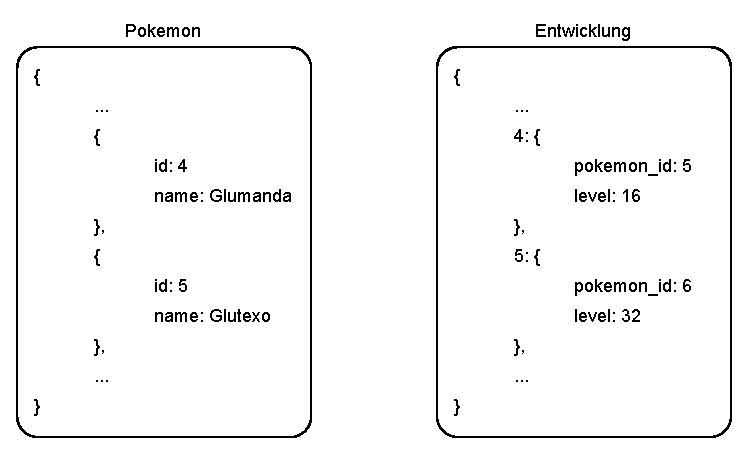
\includegraphics[width=0.75\textwidth]{pictures/example_1.pdf}
    \end{center}
\end{frame}

\begin{frame}{Tipps}
    Zuerst vergleichen wir die n-te \texttt{Pokemon.id} mit \texttt{Entwicklung.von}:

    \begin{center}
        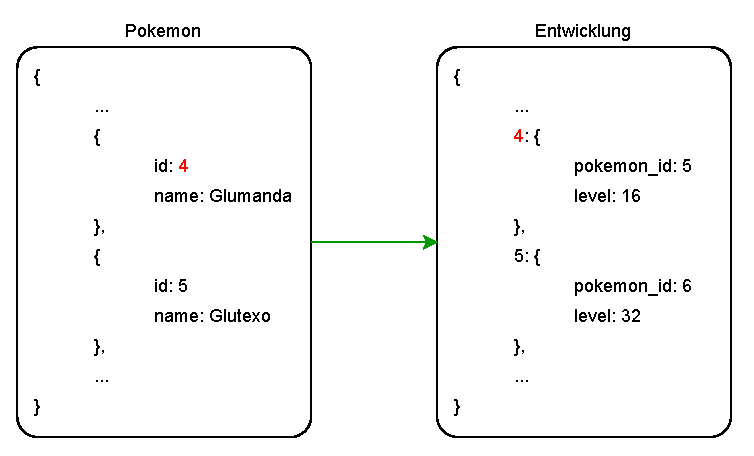
\includegraphics[width=0.75\textwidth]{pictures/example_2.pdf}
    \end{center}
\end{frame}

\begin{frame}{Tipps}
    Die erhaltene \texttt{Entwicklung.zu} finden wir in \texttt{Pokemon.id}:

    \begin{center}
        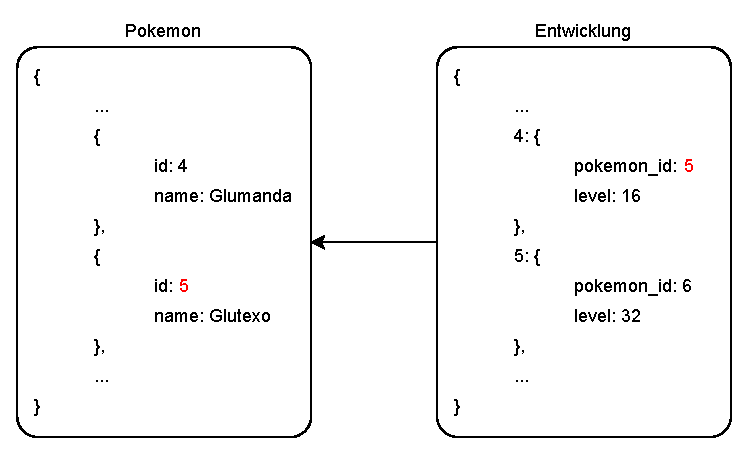
\includegraphics[width=0.75\textwidth]{pictures/example_3.pdf}
    \end{center}
\end{frame}

\begin{frame}{Tipps}
    Nun überschreiben wir das n-te Pokémon mit seiner Entwicklung:

    \begin{center}
        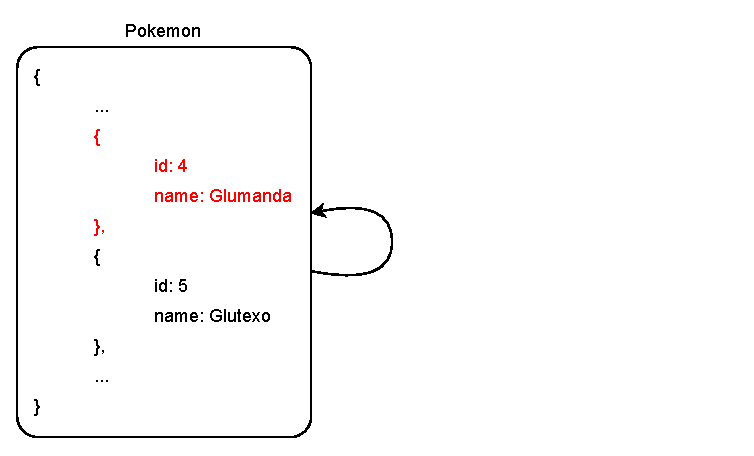
\includegraphics[width=0.75\textwidth]{pictures/example_4.pdf}
    \end{center}
\end{frame}

\begin{frame}{Tipps}
    Und erhalten:

    \begin{center}
        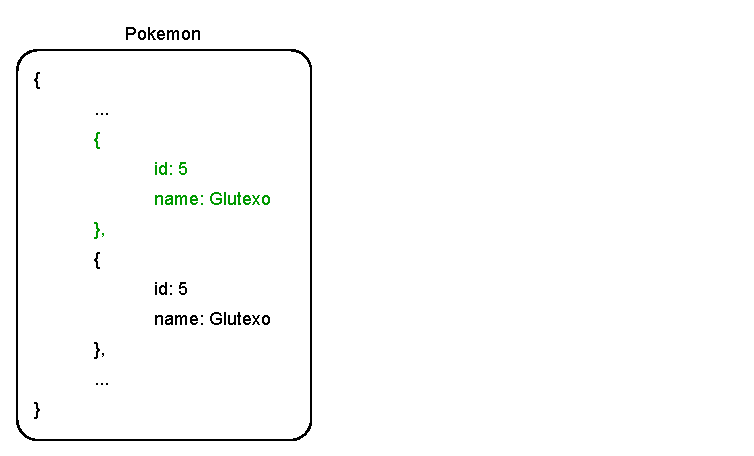
\includegraphics[width=0.75\textwidth]{pictures/example_5.pdf}
    \end{center}
\end{frame}

\begin{frame}{Tipps}
    Sollten wir das n-te Pokémon nicht finden:

    \begin{center}
        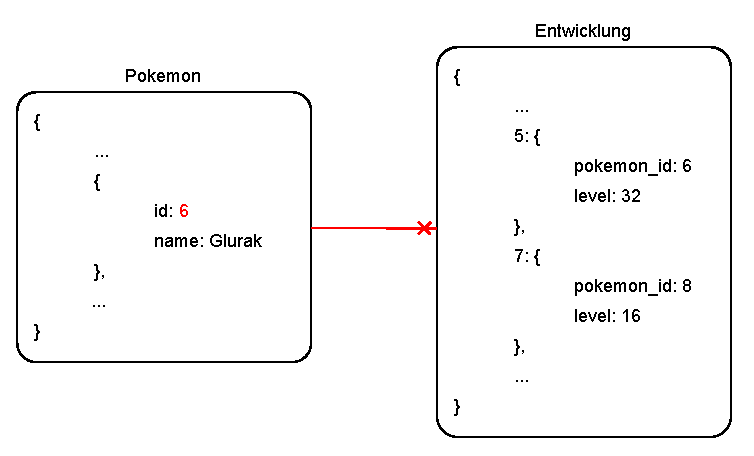
\includegraphics[width=0.75\textwidth]{pictures/example_6.pdf}
    \end{center}
\end{frame}

\begin{frame}{Tipps}
    entfernen wir dieses aus unserer View:

    \begin{center}
        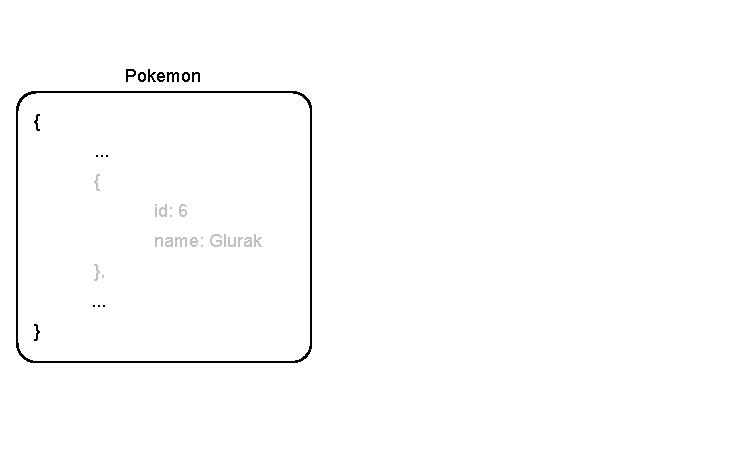
\includegraphics[width=0.75\textwidth]{pictures/example_7.pdf}
    \end{center}
\end{frame}

\begin{frame}{pokemon\_evolve\_q.cpp}
    \begin{center}
        \textbf{Code!}
    \end{center}
\end{frame}